\documentclass[a5paper,11pt]{book}
\usepackage{geometry}

\usepackage[T1]{fontenc}
\usepackage{fancyhdr}

\usepackage{amsmath}
\usepackage{amsthm}
\usepackage{amssymb}
\usepackage[spanish,es-nodecimaldot]{babel}

\usepackage{float}
% \usepackage{booktabs}
% \usepackage[bookmarks]{hyperref}

\usepackage{hyperref}
\usepackage{graphicx}

% theorems
\usepackage{thmtools}
\usepackage[framemethod=TikZ]{mdframed}
\mdfsetup{skipabove=1em,skipbelow=0em, innertopmargin=5pt, innerbottommargin=6pt}

\theoremstyle{definition}

\makeatletter

\declaretheoremstyle[headfont=\bfseries\sffamily, bodyfont=\normalfont, mdframed={ nobreak } ]{thmgreenbox}
\declaretheoremstyle[headfont=\bfseries\sffamily, bodyfont=\normalfont, mdframed={ nobreak } ]{thmredbox}
\declaretheoremstyle[headfont=\bfseries\sffamily, bodyfont=\normalfont]{thmbluebox}
\declaretheoremstyle[headfont=\bfseries\sffamily, bodyfont=\normalfont]{thmblueline}
\declaretheoremstyle[headfont=\bfseries\sffamily, bodyfont=\normalfont, numbered=no, mdframed={ rightline=false, topline=false, bottomline=false, }, qed=\qedsymbol ]{thmproofbox}
\declaretheoremstyle[headfont=\bfseries\sffamily, bodyfont=\normalfont, numbered=no, mdframed={ nobreak, rightline=false, topline=false, bottomline=false } ]{thmexplanationbox}


\declaretheorem[numberwithin=chapter, style=thmgreenbox, name=Definición]{definition}
\declaretheorem[sibling=definition, style=thmredbox, name=Corolario]{corollary}
\declaretheorem[sibling=definition, style=thmredbox, name=Proposición]{prop}
\declaretheorem[sibling=definition, style=thmredbox, name=Teorema]{theorem}
\declaretheorem[sibling=definition, style=thmredbox, name=Lema]{lemma}



\declaretheorem[numbered=no, style=thmexplanationbox, name=Demostración]{explanation}
\declaretheorem[numbered=no, style=thmproofbox, name=Demostración]{replacementproof}
\declaretheorem[style=thmbluebox,  numbered=no, name=Ejercicio]{ex}
\declaretheorem[style=thmbluebox,  numbered=no, name=Ejemplo]{eg}
\declaretheorem[style=thmblueline, numbered=no, name=Remark]{remark}
\declaretheorem[style=thmblueline, numbered=no, name=Nota]{note}

\renewenvironment{proof}[1][\proofname]{\begin{replacementproof}}{\end{replacementproof}}

\AtEndEnvironment{eg}{\null\hfill$\diamond$}%

\newtheorem*{uovt}{UOVT}
\newtheorem*{notation}{Notación}
\newtheorem*{previouslyseen}{Como ya se ha visto}
\newtheorem*{problem}{Problema}
\newtheorem*{solution}{Solución}
\newtheorem*{observe}{Observe}
\newtheorem*{property}{Propiedad}

% \pagestyle{fancy}

% \newtheorem{theorem}{Teorema}[section]
% \newtheorem{corollary}{Corolario}[theorem]
% \newtheorem{lemma}[theorem]{Lema}
%
% \theoremstyle{definition}
% \newtheorem{definition}{Definición}[section]
\renewcommand\qedsymbol{$\blacksquare$}

% 'dedication' environment: To add a dedication paragraph at the start of book
% Source: http://www.tug.org/pipermail/texhax/2010-June/015184.html
\newenvironment{dedication}
{
    \cleardoublepage
    \thispagestyle{empty}
    \vspace*{\stretch{1}}
    \hfill\begin{minipage}[t]{0.66\textwidth}
        \raggedright
    }
    {
    \end{minipage}
    \vspace*{\stretch{3}}
    \clearpage
}

% Chapter quote at the start of chapter
% Source: http://tex.stackexchange.com/a/53380
\makeatletter
\newenvironment{chapquote}[2][2em]
{\setlength{\@tempdima}{#1}%
    \def\chapquote@author{#2}%
    \parshape 1 \@tempdima \dimexpr\textwidth-2\@tempdima\relax%
\itshape}
{\par\normalfont\hfill--\ \chapquote@author\hspace*{\@tempdima}\par\bigskip}
\makeatother


% \title{Notas de Análisis Numérico}
\title{\textbf{Notas de Análisis Numérico} \\ \small con Lozano :) }
\author{Francisco Galindo}

\date{Última actualización: \today}

\begin{document}
\frontmatter

\maketitle

\begin{dedication}
    Para Yael y el Erick
\end{dedication}

\tableofcontents
\listoffigures
\listoftables


\mainmatter

\chapter{Introducción}

\begin{chapquote}{Lozano, 2024}
    ``[...] En ese sentido, el análisis numérico es como el Fortnite.''
\end{chapquote}


\section{Sobre raíces de polinomios}

Prescindiendo del grado, todo polinomio tiene asociado un grupo, y
descubró que:

\begin{quote}
    Una ecuación es soluble si y solo si, su grupo de Galois es soluble,
    entendido por ecuación soluble aquellaque puede resolverse mediante
    operaciones elementales con radicales
\end{quote}

Lo anterior se logró mediante la observación del gripo de permutaciones
de \(n\) elementos, es decir \(S_n\). Él se dio cuenta de que el primer
grupo sin soluciones es \(S_5\), por lo que ningún polinomio de grado
mayor o igual a 5 tiene una solución exacta mediante operaciones
simples.

\section{Métodos de solución de problemas}

\subsection{Métodos analíticos (exactos)}

Se trata de los métodos que permiten encontrar una solución en forma de
fórmula, permiten calcular una cantidad en función de otra. Por ejemplo:

\begin{equation}{
        ax^2 + bx + c = 0 \implies x = \frac{-b \pm \sqrt{b^2 -4ac}}{2a}
}\end{equation}

\subsection{Soluciones gráficas (cualitativas)}

Se utilizan para aproximar una solución de manera visual. No son hay
precisión, pero son fáciles de usar. Si se quieren encontrar las raíces
de la siguiente ecuación:

\begin{equation}{
        x^2 - 4 - sin(x) = 0
}\end{equation}

A primera vista no resulta posible (no lo es) hacer despejes para
encontrar los valores de \(x\) que satisfacen la ecuación. Sin embargo,
si se escribe de la siguiente manera:

\begin{equation}{
        \underbrace{x^2 - 4}_{f(x)} = \underbrace{sin(x)}_{g(x)}
}\end{equation}

Lo anterior permite tener una idea intuitiva de las raíces como las
intersecciones entre las gráficas de las funciones \(f(x)\) y \(g(x)\):

\begin{figure}[H]
    \centering
    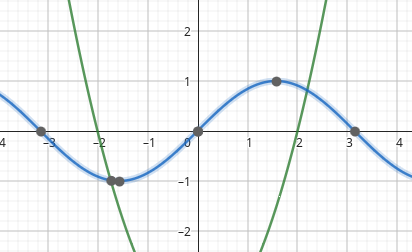
\includegraphics[width=1.0\textwidth]{img/papu.png}
    \caption{Visualización de soluciones por el método gráfico}
\end{figure}

Puede notarse así que las soluciones de la ecuación son:

\begin{equation}{
        x \approx -1.8
}\end{equation}

\begin{equation}{
        x \approx 2.1
}\end{equation}

\subsection{Métodos numéricos}

son aproximaciones a soluciones de un problema. Generalmente se basa en
la conversión del problema original utilizando operaciones aritméticas
básicas. En teoría, el resultado es tan bueno como se desee. Para el
ejemplo anterior, usando \emph{GNU Octave}, los resultados son:

\begin{equation}{
        x \approx -1.7360
}\end{equation}

\begin{equation}{
        x \approx 2.1937
}\end{equation}

\section{Exactitud y error}

¿Qué tan buenas son las soluciones obtenidas anteriormente? Para
responder esta pregunta, es importante conocer ciertas definiciones
utilizadas durante el curso.

\begin{definition}[Exactitud]
    Es el grado de proximidad de una solución para un problema dado.


\end{definition}

\begin{eg}
    Un ejemplo es esta secuencia de aproximaciones progresivamente más exactas:

    \begin{align*} 
        \pi &\approx 3 \\ 
            &\approx 3.1 \\ 
            &\approx 3.14 \\ 
            &\approx 3.141592 \\ 
    \end{align*}

\end{eg}

\begin{definition}[Precisión]
    Es la medida que indica qué tan agrupados están los valores calculados a
    su valor real. La precisión se cuantifica mediante el número de
    \emph{cifras significativas}\footnote{Las cifras significativas son
    aquellas de las que se tiene certeza en los cálculos experimentales.}
\end{definition}


\section{Tipos de errores}

Al realizar procesos numéricos, es necesario determinar una condición de
parada, un \emph{treshold} para cuando el resultado sea exacto con
cierta precisión. Los siguientes conceptos serán útiles para denotar
estas condiciones de detención:

\begin{itemize}
    \item
        \textbf{Error absoluto}: Es la diferencia entre el valor real y el
        valor calculado. Generalmente tiene unidades físicas:

        \begin{equation}{
                E_T = \text{Valor}_{\text{real}} - \text{Valor}_{\text{calculado}}
        }\end{equation}
    \item
        \textbf{Error relativo (porcentual)}: Es la medida del error absoluto
        en términos porcentuales:

        \begin{equation}{
                \varepsilon_{T} = \left| {\frac{E_T}{\text{Valor}_{\text{real}}}} \right| * 100 \%
        }\end{equation}
\end{itemize}


\begin{ex}

    En un vertedero local se reciben camiones de desechos. Por lo general,
    en estos lugares, se pesan tales camiones en básculas. Suponiendo que
    hay dos básculas y una está recién calibrada, se pesa un camión, dando
    como resultado las siguientes mediciones:

    \begin{eqnarray*}
        P_{B_1} &= 3552\text{ kg}\\
        P_{B_2} &= 3633\text{ kg}
    \end{eqnarray*}

    Suponiendo que la báscula 1 (\(B_1\)) es la calibrada, ¿cuál es el error
    absoluto y relativo de la segunda báscula?

    \begin{solution}
        Para calcular el error, se utiliza:

        \begin{equation}{
                E_T = P_{B_1} - P_{B_2} = 3552 - 3633 = -81 \text{ kg}
        }\end{equation}

        Para calcular el error relativo, se usa:

        \begin{center}
            \boxed{\varepsilon_T = \left| \frac{P_{B_1} - P_{B)_2}}{P_{B_1}} \right| * 100\% = 2.28\%}
        \end{center}

    \end{solution}


\end{ex}


\section{Series de Taylor}

La serie de Taylor tiene múltiples aplicaciones en el área teórica y
aplicada, dentro de donde destacan las siguientes:

\begin{itemize}
    \item
        Aproximar una función mediante una serie de potencias
    \item
        Linearizar ecuaciones diferenciales o integrales
    \item
        Solucionar Ecuaciones Diferenciales no lineales alrededor de un punto
        de interés
    \item
        Resolución de integrales definidas
\end{itemize}

\begin{definition}[Serie de Taylor]

    En su versión de una sola variable, la serie de Taylor de la función $f$,
    con centro en $a$, es la siguiente:

    \begin{align}
        f(x) &= f(a) + \frac{f'(a)}{1!}(x - a) + \frac{f''(a)}{2!}(x - a)^2 + ... \\
             &= \sum_{k = 0}^{\infty} \frac{f^{(k)}(a)}{k!}(x - a)^k
    \end{align}

\end{definition}


\begin{ex}
    Obtenga la serie de Taylor de la función \(f(x) = e^x\) alrededor de \(x = 0\)
\end{ex}

\begin{solution}

    Empleando directamente la definición de una serie de Taylor, con \(a = 0\):
    \begin{equation}{
            e^x = e^0 + \left[\frac{de^x}{dx}\right]_{x = 0} x + \left[\frac{d^2e^x}{dx^2}\right]_{x = 0} \frac{x^2}{2!} + \left[\frac{d^3e^x}{dx^3}\right]_{x = 0} \frac{x^3}{3!} + ...
    }\end{equation}

    Simplificando:

    \begin{equation}{
            \boxed{e^x = 1 + x + \frac{x^2}{2!} + \frac{x^3}{3!} + ...}
    }\end{equation}

\end{solution}

\begin{ex}

    Considere el péndulo representado por la figura \ref{fig:pendulo}, donde
    las únicas fuerzas actuando son la tensión de la cuerda y el peso del
    péndulo. Para escribir la posición angular del péndulo como una función del
    tiempo, uno puede apoyarse en la Segunda Ley de Newton:

    \begin{figure}[H]
        \centering
        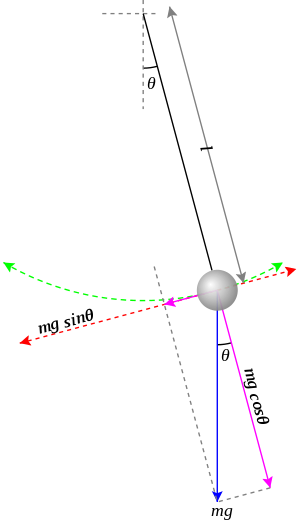
\includegraphics[height=3in]{img/pendulo.png}
        \caption{Diagrama de fuerzas de un péndulo simple.}
        \label{fig:pendulo}
    \end{figure}

    \begin{equation}
        F = ma
    \end{equation}

    Como el movimiento está restringido a una trayectoria circular, sólo es de
    interés el componente de la fuerza que es tangencial al movimiento del
    péndulo (el signo es negativo porque el ángulo siempre tiene signo
    contrario al vector de fuerza en este sistema de referencia):

    \begin{align}
        F &= -mg \sin \theta\\
        a &= -g \sin \theta\\
    \end{align}

    Considerando la siguiente relación entre la aceleración tangencial $a$ y la aceleración angular $\alpha$, donde $l$ es la longitud del péndulo:

    \begin{equation}
        \alpha = \frac{a}{l}
    \end{equation}

    Puede llegarse a la siguiente ecuación diferencial:

    \begin{align}
        l \alpha &= -g \sin \theta\\
        \alpha &= -\frac{g}{l} \sin \theta \\
        \frac{d^2 \theta}{dt^2} &= -\frac{g}{l} \sin \theta \\
        0 &= \frac{d^2 \theta}{dt^2} + \frac{g}{l} \sin \theta
    \end{align}

    Suponiendo que el péndulo oscila en ángulos pequeños (por ejemplo, que
    inicia desde el reposo con un ángulo de $\frac{\pi}{20}$), resuelva la
    siguiente ecuación diferencial:

    \begin{equation}{
            \frac{d^2 \theta}{dt^2} + \frac{g}{l} \sin \theta = 0,
            \begin{cases}
                \theta(0) = \frac{\pi}{20}\\
                \theta'(0) = 0
            \end{cases}
    }\end{equation}

    \begin{solution}

        La ecuación anterior tiene únicamente solución analítica mediante
        integrales elípticas (es necesario usar la serie del binomio). Sin
        embargo, como la oscilación inicial es pequeña, se puede aproximar el
        seno mediante series de Taylor.

        La serie de Taylor de la función seno, con centro en 0, es la siguiente:

        \begin{align}
            \sin \theta &= \theta - \frac{\theta^3}{3!} + \frac{\theta^5}{5!} - \frac{\theta^7}{7!} + ... \\  
                        &= \theta \underbrace{- \frac{\theta^3}{6} + \frac{\theta^5}{120} - \frac{\theta^7}{5040} + ...}_{\text{despreciables cuando } \theta \text{ es pequeño}} \\
                        &\approx \theta
        \end{align}

        Podemos concluir que, si el ángulo de oscilación es pequeño:

        \begin{equation}{
                \sin \theta \approx \theta
        }\end{equation}

        Sustituyendo, se obtiene la versión linearizada de la ecuación
        diferencial:

        \begin{equation}{
                \frac{d^2 \theta}{dt^2} + \frac{g}{l} \theta = 0,
                \begin{cases}
                    \theta(0) = \frac{\pi}{20}\\
                    \theta'(0) = 0
                \end{cases}
        }\end{equation}

        La solución analítica de la ecuación anterior es:

        \begin{equation}{
                \boxed{\theta_{\text{lineal}} = \frac{1}{20} \pi \cos(\sqrt{\frac{g}{l}} t)}
        }\end{equation}

    \end{solution}

    Si se compara la solución lineal con la no lineal, es posible
    observar que la aproximación es bastante acertada:

    \begin{figure}[H]
        \centering
        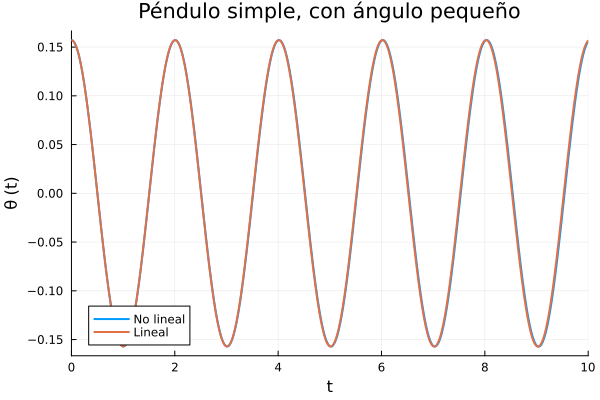
\includegraphics[width=1.0\textwidth]{img/small.png}
        \caption{Comparación de soluciones para $\theta(0) = \frac{\pi}{20}$}
        \label{fig:pendulo_sol_small}
    \end{figure}

    Sin embargo, para valores iniciales de $\theta$ más grandes, el error se
    vuelve evidente:


    \begin{figure}[H]
        \centering
        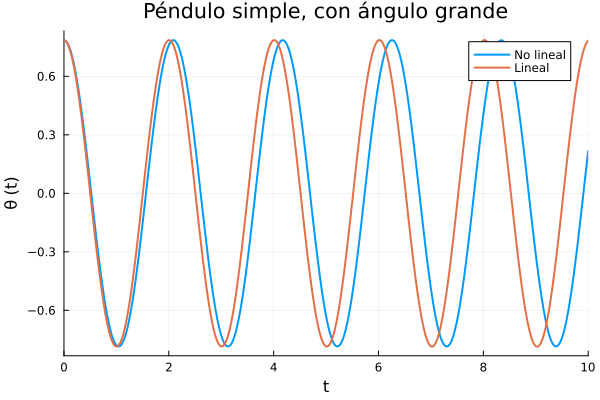
\includegraphics[width=1.0\textwidth]{img/big.png}
        \caption{Comparación de soluciones para $\theta(0) = \frac{\pi}{4}$}
        \label{fig:pendulo_sol_big}
    \end{figure}


\end{ex}



\end{document}
